\documentclass[UTF8,12pt, a4paper]{ctexart}
\usepackage{geometry}
\usepackage{listings}
\usepackage{xcolor}
\usepackage{amsmath}
\usepackage{graphicx}
\usepackage{rotating}
\usepackage{arydshln}

\geometry{left=2.0cm, right=2.0cm, top=1.0cm, bottom=2.5cm}

  \title{矩阵分析作业7:模和内积二}
  \author{2019.11.10}
  \date{}
  \begin{document}
  \maketitle
  \pagestyle{plain}
  \allowdisplaybreaks

  \subsection*{Exercise.1}

  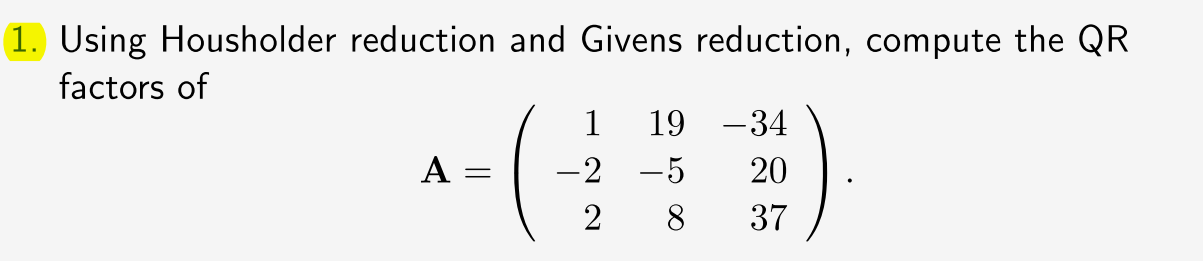
\includegraphics[scale=0.8]{question1.png} \\
  (1).Housholder约简,首先
  \begin{align*}
    A = 
    \left(
      \begin{matrix}
        &1 & 19 & -34 \\
        &-2 & -5 & 20 \\
        &2 & 8 & 37 
      \end{matrix}
    \right)
  \end{align*}

  先消去(1,1)下边的元素,
  \begin{align*}
    u_1=A_{*1}-||A_{*1}||e_1&=A_{*1}-3e_1=
    \left(
      \begin{matrix}
        &1 \\
        &-2 \\
        &2
      \end{matrix}
    \right) -
    \left(
      \begin{matrix}
        &3 \\
        &0 \\
        &0
      \end{matrix}
    \right) = 2
    \left(
      \begin{matrix}
        &-1 \\
        &-1 \\
        &1
      \end{matrix}
    \right)  \\
    R_1=I-2\frac{u_1 u_1^T}{u_1^Tu_1}=&
    I-\frac{2}{3}
    \left(
      \begin{matrix}
        &1 &1  &-1  \\
        &1 &1  &-1  \\
        &-1 &-1  &1  
      \end{matrix}
    \right)
    =\frac{1}{3}
    \left(
      \begin{matrix}
        &1 &-2  &2  \\
        &-2 &1  &2  \\
        &2 &2  &1  
      \end{matrix}
    \right)\\
    R_1A =&
    \left(
      \begin{matrix}
        &3 &15  &0  \\
        &0 &-9  &54  \\
        &0 &12  &3  
      \end{matrix}
    \right)
  \end{align*}

  下面再消去(2,2)下面的元素,
  \begin{align*}
    A_2 = &
    \left(
      \begin{matrix}
        &-9  &54  \\
        &12  &3 
      \end{matrix}
    \right) 
  \end{align*}
  \begin{align*}
    u_2=[A_2]_{*1}-||[A_2]_{*1}||e_1=
    \left(
      \begin{matrix}
        &-9 \\
        &12 
      \end{matrix}
    \right)- 15
    \left(
      \begin{matrix}
        &1 \\
        &0 
      \end{matrix}
    \right) =12
    \left(
      \begin{matrix}
        &-2 \\
        &1 
      \end{matrix}
    \right)
  \end{align*}
  \begin{align*}
    \hat{R_2}=I-2\frac{u_2 u_2^T}{u_2^Tu_2}=
    =\frac{1}{5}
    \left(
      \begin{matrix}
        &-3 &4 \\
        &4 &3
      \end{matrix}
    \right),
    \ \ \ \ and \ \ \ \ 
    \hat{R_2}A_2=
    \left(
      \begin{matrix}
        &15 &-30 \\
        &0 &45
      \end{matrix}
    \right)
  \end{align*}
  所以,
  \begin{align*}
    R_2 =
    \left(
      \begin{matrix}
        &1 &0  &0  \\
        &0 &\frac{-3}{5}  &\frac{4}{5}  \\
        &0 &\frac{4}{5}  &\frac{3}{5} 
      \end{matrix}
    \right),
    \ \ \ \  and \ \ \ \ 
    P=R_1R_2=
    \left(
      \begin{matrix}
        &\frac{1}{3} &\frac{-2}{3}  &\frac{2}{3}  \\
        &\frac{14}{15} &\frac{1}{3}  &\frac{-2}{15} \\
        &\frac{-2}{15} &\frac{2}{3} &\frac{11}{15}
      \end{matrix}
    \right)
  \end{align*}
  \begin{align*}
    PA=R_2 R_1 A=
    \left(
      \begin{matrix}
        &3 &15  &0  \\
        &0 &15 &-30 \\
        &0 &0 &45
      \end{matrix}
    \right) = T
  \end{align*}

  即$PA=T$,我们可以得到$A=P^TT$的类似于QR分解的形式,其中$Q=P^T$,上三角矩阵$R=T$。\\ \\
  (2).Givens约简,首先消去(2,1)
  \begin{align*}
    P_{12} = \frac{1}{\sqrt{5}}
    \left(
      \begin{matrix}
        &1 & -2 &0 \\
        &2 & 1 & 0 \\
        &0 & 0 & \sqrt{5} 
      \end{matrix}
    \right),
    \ \ \ \  and \ \ \ \ 
    P_{12}A=
    \frac{1}{\sqrt{5}}
    \left(
      \begin{matrix}
        &5 & 29 & -74 \\
        &0 &33 &-48 \\
        &2\sqrt{5} &8\sqrt{5} & 37\sqrt{5} 
      \end{matrix}
    \right)
  \end{align*}
  再消去(3,1)元素,
  \begin{align*}
    P_{13} = \frac{1}{3}
    \left(
      \begin{matrix}
        &\sqrt{5} & 0 &2 \\
        &0 & 3 & 0 \\
        &-2 & 0 & \sqrt{5} 
      \end{matrix}
    \right),
    \ \ \ \  and \ \ \ \ 
    P_{13}P_{12}A=
    \frac{1}{\sqrt{5}}
    \left(
      \begin{matrix}
        &3\sqrt{5} & 15\sqrt{5} & 0 \\
        &0 &33 &-48 \\
        &0 &-6 & 111
      \end{matrix}
    \right)
  \end{align*}
  再消去(3,2)的元素,
  \begin{align*}
    P_{23} = \frac{1}{5\sqrt{5}}
    \left(
      \begin{matrix}
        &5\sqrt{5} & 0 &0 \\
        &0 & 11 & -2 \\
        &0 & 2 & 11
      \end{matrix}
    \right),
    \ \ \ \  and \ \ \ \ 
    P_{23}P_{13}P_{12}A=
    \left(
      \begin{matrix}
        &3 &15  &0  \\
        &0 &15 &-30 \\
        &0 &0 &45
      \end{matrix}
    \right)
  \end{align*}
  令$P=P_{23}P_{13}P_{12}$,得
  \begin{align*}
    P=P_{23}P_{13}P_{12}=
    \left(
      \begin{matrix}
        &\frac{1}{3} &\frac{-2}{3}  &\frac{2}{3}  \\
        &\frac{14}{15} &\frac{1}{3}  &\frac{-2}{15} \\
        &\frac{-2}{15} &\frac{2}{3} &\frac{11}{15}
      \end{matrix}
    \right)
    \ \ \ \  and \ \ \ \ `'
    T=P_{23}P_{13}P_{12}A=
    \left(
      \begin{matrix}
        &3 &15  &0  \\
        &0 &15 &-30 \\
        &0 &0 &45
      \end{matrix}
    \right)
  \end{align*}
  同样可以得到$PA=T$的形式,
  所以$A=P^TT$的类似于QR分解的形式,其中$Q=P^T$,上三角矩阵$R=T$。

\subsection*{Exercise.7}
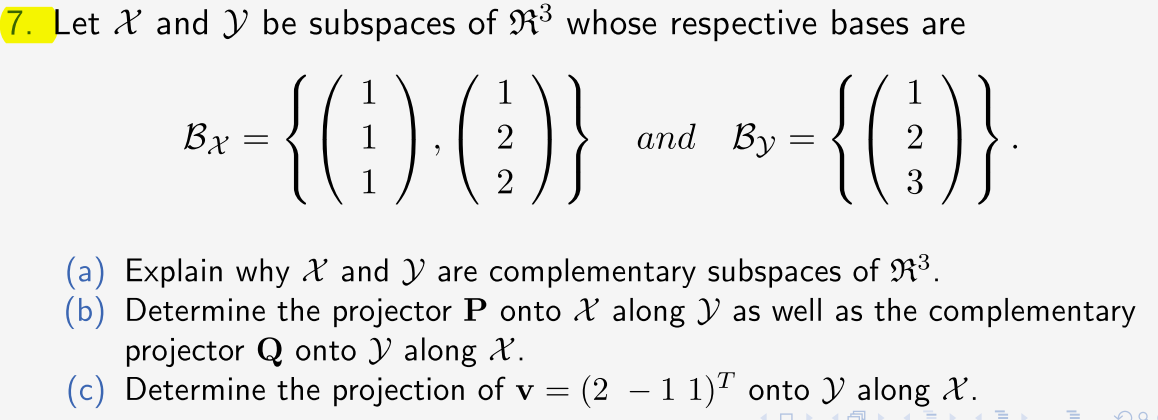
\includegraphics[scale=0.8]{question7.png}\\
(a)由题目,
\begin{align*}
  &\mathcal{B}_{\mathcal{X}} \cap \mathcal{B}_{\mathcal{Y}}=\phi \\
  \mathcal{B}=&\mathcal{B}_{\mathcal{X}} \cup \mathcal{B}_{\mathcal{Y}} = 
  \left\{
    \left(
      \begin{matrix}
        &1 \\
        &1 \\
        &1
      \end{matrix}
    \right),
    \left(
      \begin{matrix}
        &1 \\
        &2 \\
        &2
      \end{matrix}
    \right),
    \left(
      \begin{matrix}
        &1 \\
        &2 \\
        &3
      \end{matrix}
    \right)
  \right\}
\end{align*}
令A等于$\mathcal{B}$的列向量组成的矩阵,则$rank(A)=3$,、、
所以$\mathcal{B}$中三个向量构成了$\mathcal{R}^3$空间中的一组基,
因此,可以说$\mathcal{X}$和$\mathcal{Y}$构成了$\mathcal{R}^3$空间中的互补子空间。\\ \\
(b).由题,沿$\mathcal{Y}$方向到$\mathcal{X}$的投影算子$P$为,
\begin{align*}
  P=[X|0][X|Y]^{-1}=
  \left(
    \begin{matrix}
      &1 & 1 & 0 \\
      &1 & 2 & 0 \\
      &1 & 2 & 0
    \end{matrix}
  \right)
  \left(
    \begin{matrix}
      &2 & -1 & 0 \\
      &-1 & 2 & -1 \\
      &0 & -1 & 1
    \end{matrix}
  \right) = 
  \left(
    \begin{matrix}
      &1 & 1 & -1 \\
      &0 & 3 & -2 \\
      &0 & 3 & -2
    \end{matrix}
  \right) 
\end{align*}
沿$\mathcal{X}$方向到$\mathcal{Y}$的投影算子$Q$为,
\begin{align*}
  Q=I-P= 
  \left(
    \begin{matrix}
      &0 & -1 & 1 \\
      &0 & -2 & 2 \\
      &0 & -3 & 3
    \end{matrix}
  \right) 
\end{align*}
(c).由上可知,$v$沿$\mathcal{X}$方向到$\mathcal{Y}$的投影为,
\begin{align*}
  y=Qv=
  \left(
    \begin{matrix}
      &0 & -1 & 1 \\
      &0 & -2 & 2 \\
      &0 & -3 & 3
    \end{matrix}
  \right) 
  \left(
    \begin{matrix}
      &2 \\
      &-1 \\
      &1
    \end{matrix}
  \right) = 
  \left(
    \begin{matrix}
      &2 \\
      &4 \\
      &6
    \end{matrix}
  \right) 
\end{align*}
\end{document}
